\documentclass[tikz,border=2mm]{standalone}

\usetikzlibrary{arrows.meta,backgrounds,calc,chains,fit,shapes.symbols}

\begin{document}

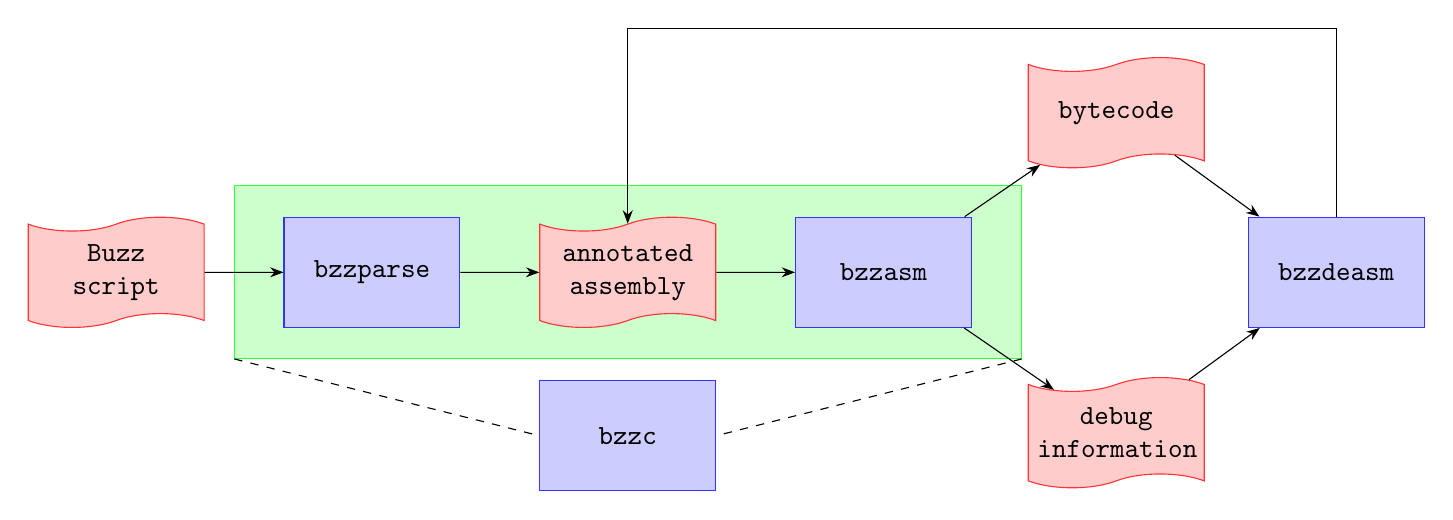
\begin{tikzpicture}[process/.style={rectangle,draw=blue!80,fill=blue!20,minimum size=1.4cm,text width=2cm,align=center,font=\tt}]

  \begin{scope}[start chain=toolset,
    node distance=1cm,
    every node/.style={draw,on chain,minimum size=1.4cm,text width=2cm,align=center,font=\tt},
    every join/.style={-Stealth},
    output/.style={tape,draw=red!80,fill=red!20}]
    \node(script)   [join,output] {Buzz\\script};
    \node(parser)   [join,process]{bzzparse};
    \node(asm)      [join,output] {annotated\\assembly};
    \node(assembler)[join,process]{bzzasm};
    
    \begin{scope}[start branch=up going {above right}]
      \node(bytecode)[join,output]{bytecode};
    \end{scope}

    \begin{scope}[start branch=down going {below right}]
      \node(debug)[join,output]{debug\\information};
    \end{scope}
    
    \node(deasm)[process,on chain=going {right=3.5cm of \tikzchainprevious},join=with toolset/up-end by {-Stealth},join=with toolset/down-end by {-Stealth}]{bzzdeasm};
    % deasm -> asm arrow
    \coordinate(p) at ($(deasm) + (-1cm, 3.1cm)$);
    \draw[-Stealth] (deasm) -- (p) -- (p -| asm) -- (asm);
  \end{scope}

  \begin{scope}[on background layer]
    % bzzcompile rectangle
    \filldraw[draw=green!80,fill=green!20] (1.5cm,-1.1cm) rectangle (11.5cm,1.1cm);
    \node(bzzc)[below=7.5mm of asm,process]{bzzc};
    \draw[dashed] (1.5cm,-1.1cm) -- (bzzc.west);
    \draw[dashed] (11.5cm,-1.1cm) -- (bzzc.east);
  \end{scope}
\end{tikzpicture}

\end{document}